%!TEX root = ../../main.tex
\begin{figure}[b!]
	\centering
	\subfloat[]{
		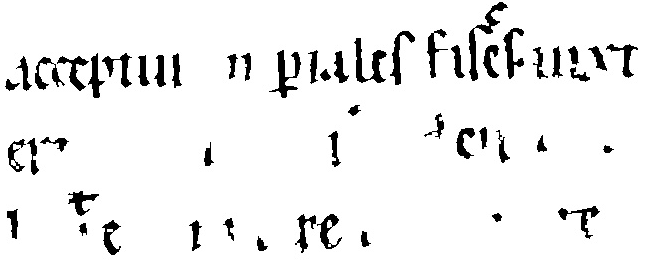
\includegraphics[width=0.45\columnwidth]{shared/img/before_lum.png}%
		\label{fig:methods:preprocessing:lumNormalization:before}%
	}
	\hfil
	\subfloat[]{
		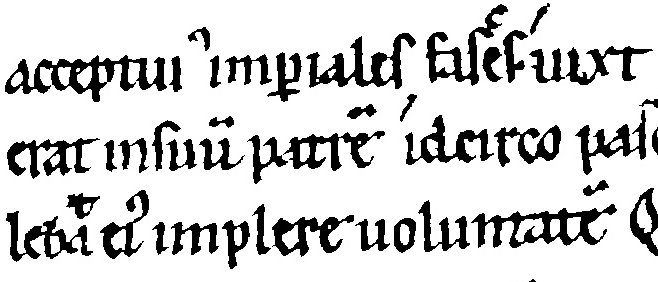
\includegraphics[width=0.45\columnwidth]{shared/img/after_lum.png}%
		\label{fig:methods:preprocessing:lumNormalization:after}%
	}
	\caption{A thresholded image with \protect\subref{fig:methods:preprocessing:lumNormalization:after} and without \protect\subref{fig:methods:preprocessing:lumNormalization:before} luminosity normalization.}
	\label{fig:methods:preprocessing:lumNormalization}
\end{figure}

The main goal of our preprocessing step is to remove noise. 
% Luminosity normalization
Luminosity normalization removes differences between images due to worn off ink, \Cref{fig:methods:preprocessing:lumNormalization} shows the results of global thresholding with and without luminosity filter. Without this normalization step most of the text would have disappeared after the global thresholding. 
% Global thresholding
We use Otsu's \cite{otsu1975threshold} method to separate the foreground from the background. 
% Opening by Reconstruction
The last preprocessing step is the removal of small components in the image, that are probably noise, via opening with a $3 \time 3$ rectangular structuring element.

